\subsection{Oppgave 4}

For oppgave 4 har vi implementert 2 funksjoner i python med numpy, én for varianten av RK4-metoden beskrevet i avsnitt 4.4, og en for varianten av RK-Fehlberg-metoden beskrevet i avsnitt 4.5 i prosjektbeskrivelsen.\newline \newline
Implementasjonen av RK4 bruker denne numeriske metoden for å finne en løsning på oppgaven: \newline

$$
\begin{aligned}
\vec{\sigma_1} &= I^{-1}W_i^T \vec{L} \\
\vec{\sigma_2} &= I^{-1}\exp{(-h\Sigma_1)}W_i^T \vec{L} \\
W_{i+1} &= W_i \exp{(\frac{h}{2}(\Sigma_1 + \Sigma_2)} \\
\text{hvor } \Sigma_i \text{ for korresponderende }& \vec{\sigma_i} \text{finnes på samme måte som } \Omega \\
\end{aligned}
$$
Koden for implementasjonen av denne numeriske metoden finnes i "kode/oppgave4/RK4.py"\newline 
Ved kjøring av koden og bruk av 10000 steg over 2 sekunder med samme initialbetingelser som i oppgave 2 ($I=Id_{3x3}, X_0 = I, \vec{L} = \begin{bmatrix} 1 & 0 & 0\end{bmatrix})$ Så får vi dette resultatet ved siste iterasjon (altså t = 2s):\newline
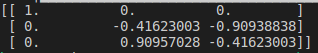
\includegraphics{rapport/resultat/bilder/oppg4_1.png}\newline
Vi kan sammenligne dette med resultatet fra eksaktløsningen \newline
\begin{equation}
    X(t)=\begin{bmatrix}1&0&0\\0&\cos t&-\sin t\\0&\sin t&\cos t\end{bmatrix}
\end{equation}
\begin{equation}
    X(2)=\begin{bmatrix}1&0&0\\0&-0.416&-0.909\\0&0.909&-0.416\end{bmatrix}
\end{equation} \newline Ser at svarene stemmer godt overens \newline \newline
Implementasjonen av RK4 tar i bruk skjemaet i ligning (39), som i koden er lagret i "kode/utils/utils.py" som matrisene A, B og c.\newline 
Stegene for den numeriske utregningen er: \newline
$$
\begin{aligned}
\vec{\sigma_1} &= I^{-1}W_i^T\vec{L} \\
\vec{\sigma_2} &= I^{-1}\exp(-ha_{21}\Sigma_1)W_i^T\vec{L} \\
\vec{\sigma_3} &= I^{-1}\exp(-h(a_{31}\Sigma_1 + a_{32}\Sigma_2))W_i^T\vec{L}  \\
\vec{\sigma_4} &= I^{-1}\exp(-h(a_{41}\Sigma_1 + a_{42}\Sigma_2 + a_{43}\Sigma_3))W_i^T\vec{L}  \\
\vec{\sigma_5} &= I^{-1}\exp(-h(a_{51}\Sigma_1 + a_{52}\Sigma_2 + a_{53}\Sigma_3 + a_{54}\Sigma_4))W_i^T\vec{L} \\
\vec{\sigma_6} &= I^{-1}\exp(-h(a_{61}\Sigma_1 + a_{62}\Sigma_2 + a_{63}\Sigma_3 + a_{64}\Sigma_4 + a_{65}\Sigma_5))W_i^T\vec{L}  \\
W_{i+1} &= W_i\exp(h(b_{11}\Sigma_1 + b_{12}\Sigma_2 + b_{13}\Sigma_3 + b_{14}\Sigma_4 + b_{15}\Sigma_5 + b_{16}\Sigma_6)) \\
Z_{i+1} &= W_i\exp(h(b_{21}\Sigma_1 + b_{22}\Sigma_2 + b_{23}\Sigma_3 + b_{24}\Sigma_4 + b_{25}\Sigma_5 + b_{26}\Sigma_6)) \\
\Delta W &= W_{i+1} - Z_{i+1} \\
E &= \sqrt{trace(\Delta W^T \Delta W)}
\end{aligned}
$$
For hvert ledd i tillegg til å finne W finner vi da også et tilnærmet mål på feilen i utregningen av $W_{i}$ og lagrer disse feilene i en liste E.\newline \newline
Koden for implementasjonen av RK-Fehlberg ligger i "kode/oppgave4/RK45.py".\newline
Ved kjøring av koden og bruk av 10000 steg over 2 sekunder med samme initialbetingelser som i oppgave 2 ($I=Id_{3x3}, X_0 = I, \vec{L} = \begin{bmatrix} 1 & 0 & 0\end{bmatrix})$ Så får vi dette resultatet ved siste iterasjon (altså t = 2s):\newline
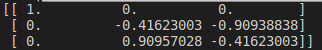
\includegraphics{rapport/resultat/bilder/oppg4_2.png}\newline

Dette stemmer godt overens med eksaktløsningen: \newline
\begin{equation}
    X(2)=\begin{bmatrix}1&0&0\\0&-0.416&-0.909\\0&0.909&-0.416\end{bmatrix}
\end{equation}